\documentclass{book}
\usepackage{graphicx, geometry, xcolor, fancyvrb, hyperref, ulem, microtype}
\geometry{a5paper, left=20mm, right=20mm, top=10mm}
\begin{document}
\pagecolor{black}
\color{white}% set the default colour to
\clearpage
%% temporary titles
% command to provide stretchy vertical space in proportion
\newcommand\nbvspace[1][3]{\vspace*{\stretch{#1}}}
% allow some slack to avoid under/overfull boxes
\newcommand\nbstretchyspace{\spaceskip0.5em plus 0.25em minus 0.25em}
% To improve spacing on titlepages
\newcommand{\nbtitlestretch}{\spaceskip0.6em}
\begin{center}
\bfseries
\nbvspace[1]
\Huge
{\nbtitlestretch\huge
    \textbf{FASCISM}: 100 QUESTIONS ASKED AND ANSWERED}

\nbvspace[1]
\normalsize
    \textit{
``REAL FREEDOM MEANS GOOD WAGES,\\
SHORT HOURS, SECURITY IN EMPLOYMENT''\\
}
\nbvspace[1]
\small BY\\
    \Large SIR OSWALD MOSLEY\\[0.5em]

\nbvspace[2]

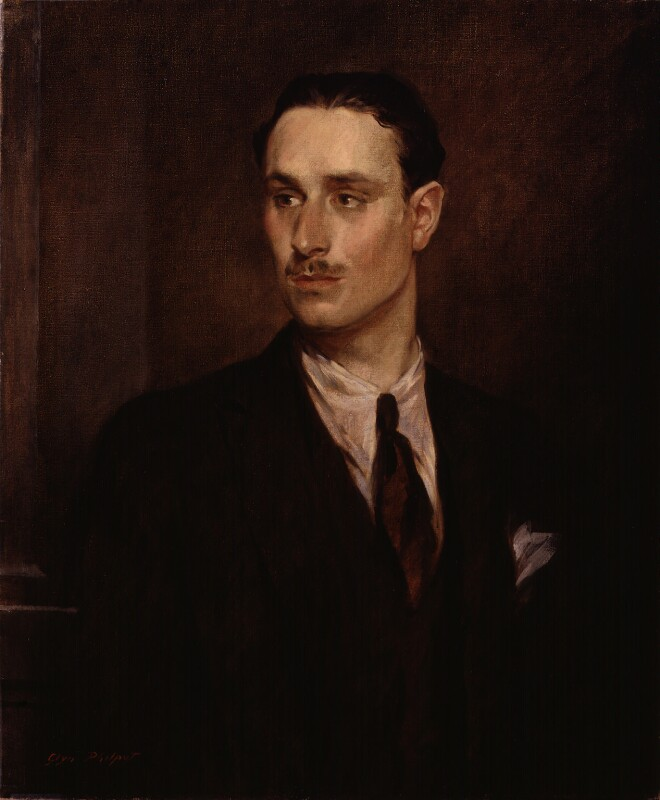
\includegraphics[width=3.1in]{./img/1.jpg}
\nbvspace[3]
\normalsize

1936\\
\large
    \textit{Mosley Revisited}
\nbvspace[1]
\end{center}
\newpage
\pagenumbering{gobble}
\pagecolor{white}
\color{black}
\begin{theindex}
 \item Economy
  \subitem
 \item Religion
  \subitem 10.5,
 \item Democracy
 \item Personal
     \subitem \textbf{2}.\textit{1},
 \item General
     \subitem \textbf{4}.\textit{2}, \textbf{5}.\textit{2},
\indexspace
For quick navigation the index key is as follows...
    \textbf{10}.\textit{1}. Bold numbers refer to Question number
    while italicised numbers refer to page number.
\\\\
    This index aims to categorise each question into its respective field. Some questions are more niche or do not fit the major categories therefore have been placed in general.
\end{theindex}
\newpage
\pagenumbering{arabic}
\pagestyle{plain}
\pagecolor{white}
\color{black}
\begin{flushright}
\textbf{1. What is the attitude of the B.U.F. towards the Crown?}
Absolute loyalty to the Crown. We shall in every way maintain its
dignity.
\end{flushright}
\begin{flushleft}
\textbf{2. Why did you leave the Socialist Party?}

For the same reason that I left the Conservative Party, namely that it had broken every pledge it
ever gave. I entered Parliament as the youngest member after the war. I was Conservative
because that Party had been loyal to the country in the war and advanced a great programme of
Social Reform. ``A land fit for heroes to live in'' is a bitter mockery in the light of the subsequent
betrayal, but it was a living reality to my generation at the end of the war. That conception went
down in the triumph of the war profiteers who comprised the majority of the post-war Parliament.
I left the Conservative Party and fought and beat them twice as an Independent in their old
stronghold at Harrow. Independence appeared to me to be sterile in service to the country, and I
joined the Labour Party, which then presented the only hope of any effective action despite its
many and obvious defects.

For seven years I worked hard for Labour, and in 1929 we came to office on a pledge to tackle
unemployment. I was one of the three Ministers charged with that great task. For a year the
Government would do nothing. At the end of a year I produced a plan I had worked out within
the Departments for giving immediate work to 800,000 men and women, and a further long term
policy for the reconstruction of British industry in accord with modern facts. I said to the
Government ``Either accept this plan or produce a better one of your own.'' They would do
neither, and I resigned. I took the issue to the Parliamentary Party warning them of the coming
crisis which arrived eighteen months later. Out of 290 only 29 voted with me. I took the issue to
the Party Conference and over a million voted with me, but the big block vote in the hands of the
Trade Union bosses voted us down. I then turned my back for ever on the old system and began
the long and hard struggle to create from nothing the new force capable of winning a new
civilisation.

The Labour Party, including the present Leaders, clung to their offices for another year, while the
unemployment figures mounted by over a million until the bankers knocked them on the head
like the tame cattle they were. These men climbed to great positions on the shoulders of the
workers, only to betray them for office and power. It was right to give both the old Parties a
chance to make good - I shall never regret it. If I and millions of others had not given them that
chance our case for a new Movement would not now be so strong. The fact that I have belonged
to both the old Parties is often urged against me. I regard it as one of the strong points in my case
and am prepared to argue it before any tribunal of my countrymen. For they too have trusted the old Parties and have been betrayed by them.
\end{flushleft}

\begin{flushright}
\textbf{3. How could the Labour Party carry out their Policy
    when they had not a majority?}

The simple and conclusive answer is another question. If they had an unemployment policy, why
did they not present it to Parliament? If they had been defeated they could have gone back to the
country and swept it at a General Election. They had neither a policy to present nor the courage to fight.
\end{flushright}

\begin{flushleft}
\textbf{4. Why is the movement called Fascist?}

Fascism is the name by which the modern Movement has come to be known in the world. It
would have been possible to avoid misrepresentation by calling our Movement by another name.
But it was more honest to call it Fascism and thus to let everyone know exactly where we stood.
It is up to us to defeat misrepresentation by propaganda and explanation of the real policy and
method of Fascism as it will operate in Britain. In the long run straightforward dealing is not
only honest but also pays best. The alternative name for the modern Movement is the National
Socialism used in Germany. But the German Movement also is known throughout the outside
world as Fascist, which is the name commonly used to describe the phenomenon of the modern
Movement whether in Britain, Germany or Italy. National Socialism and Fascism in my view are
the same Movement, finding different expressions in different countries in accord with different
national and racial characteristics. For seven years in the Labour Party before founding Fascism in Britain, I fought for a National
Socialist Policy in contradistinction to the International Socialism
of that Party.
\end{flushleft}

\begin{flushright}
\textbf{5. If you do not copy foreign ideas, why do you (1) wear a black shirt, (2) use the Italian
    Fascist salute, (3) use the Italian Fasces?}

(1) We wear a Blackshirt because the colour Black best expresses the iron determination of
Fascism in the conquest of red anarchy. Symbolism in itself is nothing new in British politics.
The Conservatives, who are naturally rather shy about their creed, wear a modest primrose once
a year in memory of Mr. Disraeli. The Liberals wear rosettes of varying hues at election time.
The Socialists wore red ties until they faded pink after the last Labour Government. In
symbolism as in our creed we are more full-blooded people and, literally as well as
metaphorically, have put our shirt on Fascism. Our members are not compelled to wear the
Blackshirt. In most districts only about 1 in 20 wear it. But those who have worn the Blackshirt
in the early days and publicly proclaimed their faith before the world, have performed a service
to Fascism which will never be forgotten. Strongly held opinions, strongly expressed, are a
necessity in the chaos of a flabby age. The Blackshirt, therefore, is the symbol of Fascism.

(2) The salute is not Italian nor is it German, but the Germans also use it. It is the oldest salute of
European civilisation and was used in early Britain many centuries before a Fascist Party was
created in Italy.

(3) The Fasces, too, are a symbol used in Britain for the last 2,000 years and are to be found on
most of our great monuments. The symbol was brought to Britain by our Roman ancestors, who
were here for four centuries and their stock remained for ever. The Fasces were the symbol of the
Roman Empire. What more fitting than that they should be used by the Empire which succeeded and surpassed the Roman Empire?
\end{flushright}

\begin{flushleft}
    \textbf{6. What does the flash and circle mean?}

This is our modern symbol which belongs exclusively to British Fascism. It portrays the flash of
action in the circle of unity. National action can only come from national unity, which in its turn can only come from Fascism that ends the strife
of Parties.
\end{flushleft}
\begin{flushright}
\textbf{7. What are the differences between Fascism in Britain
    and Fascism in Italy and Germany}

The main difference is that they are Italian or German and that we are British. From this all other
differences follow. Fascism in essence is a national creed finding a different national expression
and method in each nation. For this reason, Fascist Movements in' each country vary more than
Socialist or Communist Movements, which are international. All great Movements have been
common to the world as a whole, both political and religious. All the old Parties have their
foreign counterparts. Liberalism, for instance, deluged the continent with blood, but came to
Great Britain by British methods characteristic of this nation's ordered greatness. In this respect
we do what our forefathers did before us. We seek to bring the creed of our age to Great Britain
by British methods in accord with British character. We seek also to emulate their example by
finding for the creed of our age its highest expression and development in these islands. The
British have not always originated the creed of the age, but they have usually perfected it. We
claim that the policy of Fascism in Britain goes far beyond any continental analogy in
constructive conception.
\end{flushright}

\begin{flushleft}
\textbf{8. How are you going to break down the barriers of class?}
By establishment of the principle of no reward without service, and the consequent elimination
of the parasite who creates the barrier of social class. Functional differences will exist according
to difference of function, but differences of social classes will be eliminated. They arise from the
fact that in present society the few can live in idleness as a master class upon the production of
the many. Under Fascism all will serve in varying manner and degree the nation to which all are
responsible.
This present conception of divided social classes invades even productive spheres. With the
abolition of a parasitic class by our proposals for dealing with hereditary wealth, this tendency
too, will be eliminated. The Managing Director of a business will perform a different function
from that which the Charwoman performs in sweeping out his office. But the difference will be
functional and not social. Outside the difference of function and of service the Fascist State
recognises no difference between its citizens. The recognition of functional differences, however,
marks another difference between Fascism and Socialism. The equalitarian doctrines of the latter,
which are not only social but functional, lead logically to the performance of the Managing
Director's function by a committee of Charwomen.
We believe everywhere in the Leadership principle and the functional differentiation which
allocates definite responsibility to the individual. This principle rests on an obvious fact of
human nature which Socialism ignores. Men and women are born with varying gifts and
capacities.
\end{flushleft}
\begin{flushright}
\textbf{9. What about Freedom?}

At present the mass of the people have no freedom. Under Fascism for the first time they will
have freedom. What is the use of a vote if the people never get what they vote for? How can
they get what they vote for when only two big Bills can be carried through Parliament in a whole
year on account of obstruction? The beginning of freedom for the people is that the programme
for which they vote shall be carried out. It cannot be carried out until the Government has power
to act. By giving" Government the power to act, Fascism brings not the end of freedom but the
beginning of freedom. Real freedom is economic freedom. Economic freedom cannot come until
economic chaos ends ; and it cannot end until a Government has power to act.
Real freedom means good wages, short hours, security in employment, good houses, opportunity
for leisure and recreation with family and friends. Modern Science enables us to build such a
civilisation. It is not built, because Democracy prefers talk to action. We have to choose between
the freedom of a few professional politicians to talk and the freedom of the people to live. In
choosing the latter, Fascism makes freedom possible and releases the people from the economic slavery rivetted upon them by the
Democracy of talk.
\end{flushright}
\begin{flushleft}
\textbf{10. What is your attitude towards religion?}

We believe in complete religious toleration. The Fascist attitude is well summarised by the
Christian precept " Render unto Caesar the things that are Caesar's and unto God the things that
are God's."
We are concerned with the business of the Nation, not with the business of religion. None of the
great religions preach the subversion of the State, and therefore they have no conflict with
Fascism. On the contrary we welcome religion which inculcates a sense of service and of spiritual values, for service and the values
of the spirit are the essence of Fascism.
\end{flushleft}

\begin{flushright}
\textbf{11. Will there be freedom of the Press under Fascism and
    will newspapers be free to criticise the Government?}

The Press will not be free to tell lies. That is not freedom for the people but a tyranny over their
minds and souls. Much humbug is talked on this subject. What is Press freedom ? In practice it
means the right of a few millionaires to corner newspaper shares on the stock exchange and to
voice their own opinions and interests irrespective of the truth or of the national interest.

Newspapers are not made any longer by news or journalism. They are made by sheer weight of
money expressed in free gift schemes, etc. They serve not the interests of the many but the
vested interests of the few. In that service they will stoop to any lie or any debauch of the public
mind. This must be stopped, and the freedom of the National Press to serve great interests at the
expense of the nation must be curtailed. On the other hand, local newspapers, generally speaking,
are fairly conducted, with a sense of national responsibility and will certainly be treated
differently by Fascism from the great dope machines of the vested interests which now are
dignified by the undeserved title of National Press.

Constructive criticism will always be welcomed by Fascist Government. False and malicious
criticism designed to serve vested interests will be dealt with as follows. The Government
representing the Nation will have the same right to sue a newspaper which makes untrue
statements about it, as an individual at present possesses. If an individual is libelled he has
redress in the Courts. But the Nation has no redress. Any lie may be told by a newspaper,
however damaging to the national interest, with complete impunity. Lies against the nation
should be dealt with even more severely than lies against the individual. Therefore, the right to
sue in the Courts should be extended to the Nation represented by its elected Government. Press attacks on the Crown and Royal family will be regarded as an extremely serious offence. In brief,
our Press policy is that newspapers shall tell the truth. The principle is novel but who can say that it is wrong?
\end{flushright}

\begin{flushleft}
\textbf{12. What will a Fascist Government do about D.O.R.A. and similar restrictions?}

Fascism will ``substitute the obligations of manhood for the restrictions of childhood.'' We are
opposed to the present treatment of the nation as a race of children. We will sweep away this
legislation by a Parliament of old women for the protection of a minority of degenerates from
themselves. Men cannot be made sober by act of Parliament. They can only be made worthy
citizens of a great Empire by the creation of a new social sense and a higher patriotism. Fascism
teaches men and women ``to live like athletes'' in order to fit themselves for service of their
country. There will be fewer drunkards and degenerates under Fascism because there will be no
room for them in a higher civilisation. But there will also be a far greater measure of private
freedom for the normal man and woman. In their public life we ask of men a greater obligation and a higher service. In private life in return
we accord them a greater freedom.
\end{flushleft}
\begin{flushright}
\textbf{13. Will free speech be allowed such as is enjoyed to-day
    by Parties in opposition to the Government?}

When the Parties come to an end, their methods will also come to an end. But in place of that
obsolete system the people will possess a much more real freedom of speech than they enjoy to-
day. The people have no freedom of speech to-day except in private conversation, which gets
them nowhere. Only the organised Parties can afford to take halls for meetings, and only
professional talkers from Westminster do the talking. The liberty of professional talkers to talk
for ever while the Nation perishes will certainly be curtailed. But idle faction will be replaced by
opportunity for the whole people to express their opinions, and to help the Government with
constructive criticism in the great corporations constituted for that purpose. Within the
appropriate corporation every farmer or farm-worker, every engineer and miner, every doctor
and accountant, every housewife in the special corporation for married women, will be invited to
express their opinion and their suggestions will be welcomed. That is real freedom of speech.
\end{flushright}

\begin{flushleft}
\textbf{14. Will Fascism allow opposition parties to exist?}

It is the deliberate aim of Fascism to bring to an end the Party game which we believe to be the
ruin of the Nation. We substitute a new system of action suited to the modern age for the system
of talk which belongs to the past. For instance, a Parliament elected under Fascism will be a
technical and not a political Parliament. The franchise will be occupational and not geographical.
Men and women will vote according to their industry or profession, and not according to their
locality. They will vote for people versed in the problems of their industries, and not for
professional politicians. In such a system there is no place for parties and for politicians. We
shall ask the people for a mandate to bring to an end the Party system and the Parties. We invite
them to enter a new civilisation. Parties and the Party game belong to the old civilisation, which has failed.
\end{flushleft}

\begin{flushright}
\textbf{15. What about Dictatorship?}

The Fascist Movement represents Leadership, not Tyranny. It offers to the people a Leadership
in national revival which they will accept of their own free will. The Dictatorship is a
Dictatorship of the will of the people expressed through a Leadership and Government of their
own choice. The only way in which the will of the people can be carried out is through a
Leadership which they choose for the purpose and give the power to act.

Fascism offers that Leadership through which the will of the people can be effective. Thus a
Dictatorship of the people themselves replaces the present Dictatorship of Vested Interests.
Parliament and Government are paralysed by universal talk. Programmes for which the people
have voted are never implemented. As a result real Government under Democracy rests in the
hands of the great interests, such as International Finance. Fascism restores to power the people.
That power can only be expressed through Leadership voluntarily accepted and chosen, but
armed by the people with power to do what they want done.
\end{flushright}

\begin{flushleft}
    \textbf{16. How will you gain power?}

By legal and constitutional means. We seek power by the winning of a Parliamentary majority.
Directly we have completed our election machinery we shall contest Parliamentary elections.
Our first task was to create the Fascist Movement. Our second task is to create an election
machine, which in Britain is a highly technical process. When this second stage is complete we
shall fight elections.
\end{flushleft}

\begin{flushright}
\textbf{17. How will you use Parliamentary power?}

The first Act of a Fascist majority will be to confer on Fascist Government the power to act by
Order, subject to the right of Parliament at any time to dismiss the Government by vote of
censure if it abuses that Power. Thus we shall combine the power of the Government to act with the right of the people to control the
Government through the Parliament they have elected.
\end{flushright}


\begin{flushleft}
\textbf{18. If a Government has the power to act by order does it
    then injure the freedom of Debate and the right of minorities?}

The present system ignores the fact that majorities also have their rights. In the name of free
debate a minority now has the power to prevent a Government carrying out the programme for
which the majority of the people have voted. The first necessity is to secure the right of the
majority to the action which they demand by their vote. This is impossible so long as an
obstructive opposition has the power by endless talk to prevent action by Government. The will
of the people is greater than the right of the minority. That first principle is denied by the practices of present Democracy.
\end{flushleft}


\begin{flushright}
\textbf{19. How do the people retain control of a Fascist Government after giving it ``power of
action by order''?}

(1) The Parliament they have elected can at any time dismiss it by vote of censure. In this respect
they retain the same control as they at present possess.
(2) At the end of a normal lifetime of a Parliament or a lesser period they can themselves dismiss
it by a direct vote on universal franchise. The most effective control the people can possess is that any Government will have this possibility in mind.
\end{flushright}


\begin{flushleft}
\textbf{20. Should a Fascist Government incur a Parliamentary vote of censure, what occurs?}

If a Fascist Government incurs a Parliamentary vote of censure in its first Parliament, it will
immediately ask for a vote of the whole people in universal franchise whether it goes or carries
on. After the election of the second Parliament, which will be a technical and not a political
Parliament, the life of the Government will depend, not on Parliament, but on direct votes of the
whole people taken at intervals of not longer than five years. In practice we shall probably ask
for a vote of the people even more frequently, because to carry through the Fascist revolution we
shall want always to know that we have not only the tacit consent, but the enthusiastic support of
the people behind us. The support of the people is far more necessary to a Government of action
than to a Democratic Government, which tricks the people into a vote once every five years on
an irrelevant issue, and then hopes the Nation will go to sleep for another five years so that the Government can go to sleep as well.
\end{flushleft}

\begin{flushright}
\textbf{21. If the people vote against a Government what will happen?}

The Government will resign and H.M. The King will send for fresh Ministers, who, in his
opinion, will secure the confidence of the country. A fresh vote will then be taken to discover
whether or not the people have confidence in the new Government. In this way we restore the
Royal Prerogative to send for new Ministers in the event of the defeat of a Government. By
present practice the King is bound to send for the Leaders of the Parliamentary Opposition, and,
\end{flushright}

\begin{flushleft}
\textbf{22. At the end of the first Fascist Parliament how would Governments be chosen and
    Parliaments elected?}

The first Fascist Parliament will come to an end within the normal lifetime of a present
Parliament, and before that date the permanent Fascist system will be introduced. Thereafter the
life of Government will depend, not on Parliament, but on the direct vote of the whole people by
universal franchise. Nothing shall come between Government and People. They will be asked
whether or not a Government shall continue in a direct "Yes" or "No" decision. Parliament will
be elected to advise Government on the technical problems of a technical age. Therefore, it will
be elected not on a geographical but on an occupational franchise, according to industry or
profession. Parliament will become a serious body suited to the complex problems of the modern
age, and the knock-about frivolity of the Party game will be eliminated.
\end{flushleft}

\begin{flushright}
\textbf{23. When the first Fascist Government introduces a Bill to confer power of action by order
    on the Government, what will you do if the House of Lords throws it out?}

The people will have voted for a Government returned with a constitutional majority to pass this
measure as its first Act. If the House of Lords throw out the Bill under these circumstances it will
violate not only the spirit but also the practice of the British Constitution in modern times. The
Peers will be rebels against Crown and People and will be treated as such. Fascism, therefore,
would grasp the nettle and would suppress the House of Lords. It would immediately be replaced
by a Second Chamber truly representative of Modern Britain.
\end{flushright}

\begin{flushleft}
\textbf{24. }
\end{flushleft}
\end{document}
